\documentclass[a4paper, 12pt]{article}
\usepackage{geometry}
\geometry{a4paper,
total={170mm,257mm},left=2cm,right=2cm,
top=2cm,bottom=2cm}

\usepackage{mathtext}
\usepackage{amsmath}
\usepackage[utf8]{inputenc}
\usepackage[english,russian]{babel}
\usepackage{graphicx, float}
\usepackage{gensymb}
\usepackage{tabularx, colortbl}
\usepackage{caption}
\usepackage{subcaption}
\usepackage{wrapfig}
\captionsetup{labelsep=period}

\newcommand{\parag}[1]{\paragraph*{#1:}}
\DeclareSymbolFont{T2Aletters}{T2A}{cmr}{m}{it}
\newcounter{Points}
\setcounter{Points}{1}
\newcommand{\point}{\arabic{Points}. \addtocounter{Points}{1}}
\newcolumntype{C}{>{\centering\arraybackslash}X}

\author{Калинин Даниил, Б01-110}
\date{\today}
\title{Лабораторная работа 1.2.4.\\Определение главных моментов инерции твердых тел с помощью крутильных колебаний}

\begin{document}
\maketitle

\parag {Цель работы}
Измерить периоды крутильных колебаний рамки при различных положениях закрепленного в ней тела, проверить теоретическую зависимость между периодами крутильных колебаний тела относительно различных осей для каждого тела, по ним найти главные моменты инерции тел и построить эллипсоид инерции.
\parag {В работе используются}
установка для получения крутильных колебаний, набор исследуемых тел, секундомер.
\parag {Теоритическая справка} ~\\
Инерциальные свойства твердого тела при вращении определяет не только величина его массы, но и ее пространственное распределение. Последнее характеризует физическая величина, которая называется тензором инерции. Тензор инерции твердого тела может быть представлен симметричной матрицей, которая полностью определяется заданием 6 элементов. Если для какой-либо системы координат изестны все 6 элементов матрицы, то момент инерции тела относительно произвольной оси может быть вычислен по следующей формуле:

\begin{equation}
    I = I_{11}s_{1}^2 + I_{22}s_{2}^2 + I_{33}s_{3}^2 + 2I_{12}s_{1}s_{2} + 2I_{23}s_{2}s_{3} + 2I_{31}s_{3}s_{1}, 
\end{equation}

где
$s$ -- единичный вектор, а $x_i$ -- компоненты радиус-вектора и:
\begin{align}
\begin{split}
    I_{11} = \int  (x_2^2 + x_3^2) \,dm  ,\quad & I_{12} =  -\int  x_1x_2 \,dm   \\
    I_{22} = \int  (x_3^2 + x_1^2) \,dm  ,\quad & I_{23} =  -\int  x_2x_3 \,dm    \\
    I_{33} = \int  (x_1 + x_2^2) \,dm  ,\quad & I_{31} =  -\int  x_3x_1 \,dm    \\    
\end{split}
\end{align}



Как и всякая симметричная матрица, тензор инерции может быть представлен в диагональном виде. Диагольные элементы $I_x$, $I_y$, $I_z$ которого называются главными моментами инерции тела. Геометрическим представлением тензора инерции является эллипсоид инерции, уравнение которого в главных осях имеет вид:
\begin{equation}
    I_xx^2 + I_yy^2 + I_zz^2 = 1.
\end{equation}

Если начало координат совпадает с центром масс тела, то эллипсоид называется центральным.

Знание эллипсоида инерции позволяет найти момент инерции тела относительно любой оси проходящей через центр тела. Для этого необходимо провести вдоль выбранной оси радиус-вектор $\overrightarrow{r}$ до пересечения с поверхностью эллипсоида. Длина $r$ будет определять момент инерции тела относительно этой оси:
\begin{equation}
    I = \frac{1}{r^2}.
\end{equation}

Период крутильных колебаний рамки с телом определяется формулой:
\begin{equation}
    T = 2\pi\sqrt{\frac{I+I_p}{f}}
    \label{eq:period}
\end{equation} 
Где $I$, $I_p$ -- моменты инерции тела и рамки относительно оси вращения, $f$ -- модуль кручения проволоки.

На рисунке \ref{pic:parallelepiped} показано, как проходят оси вращения в параллелепипеде. Оси $AA'$, $BB'$ и $CC'$ являются главными осями данного тела.

\begin{wrapfigure}{l}{7cm}
	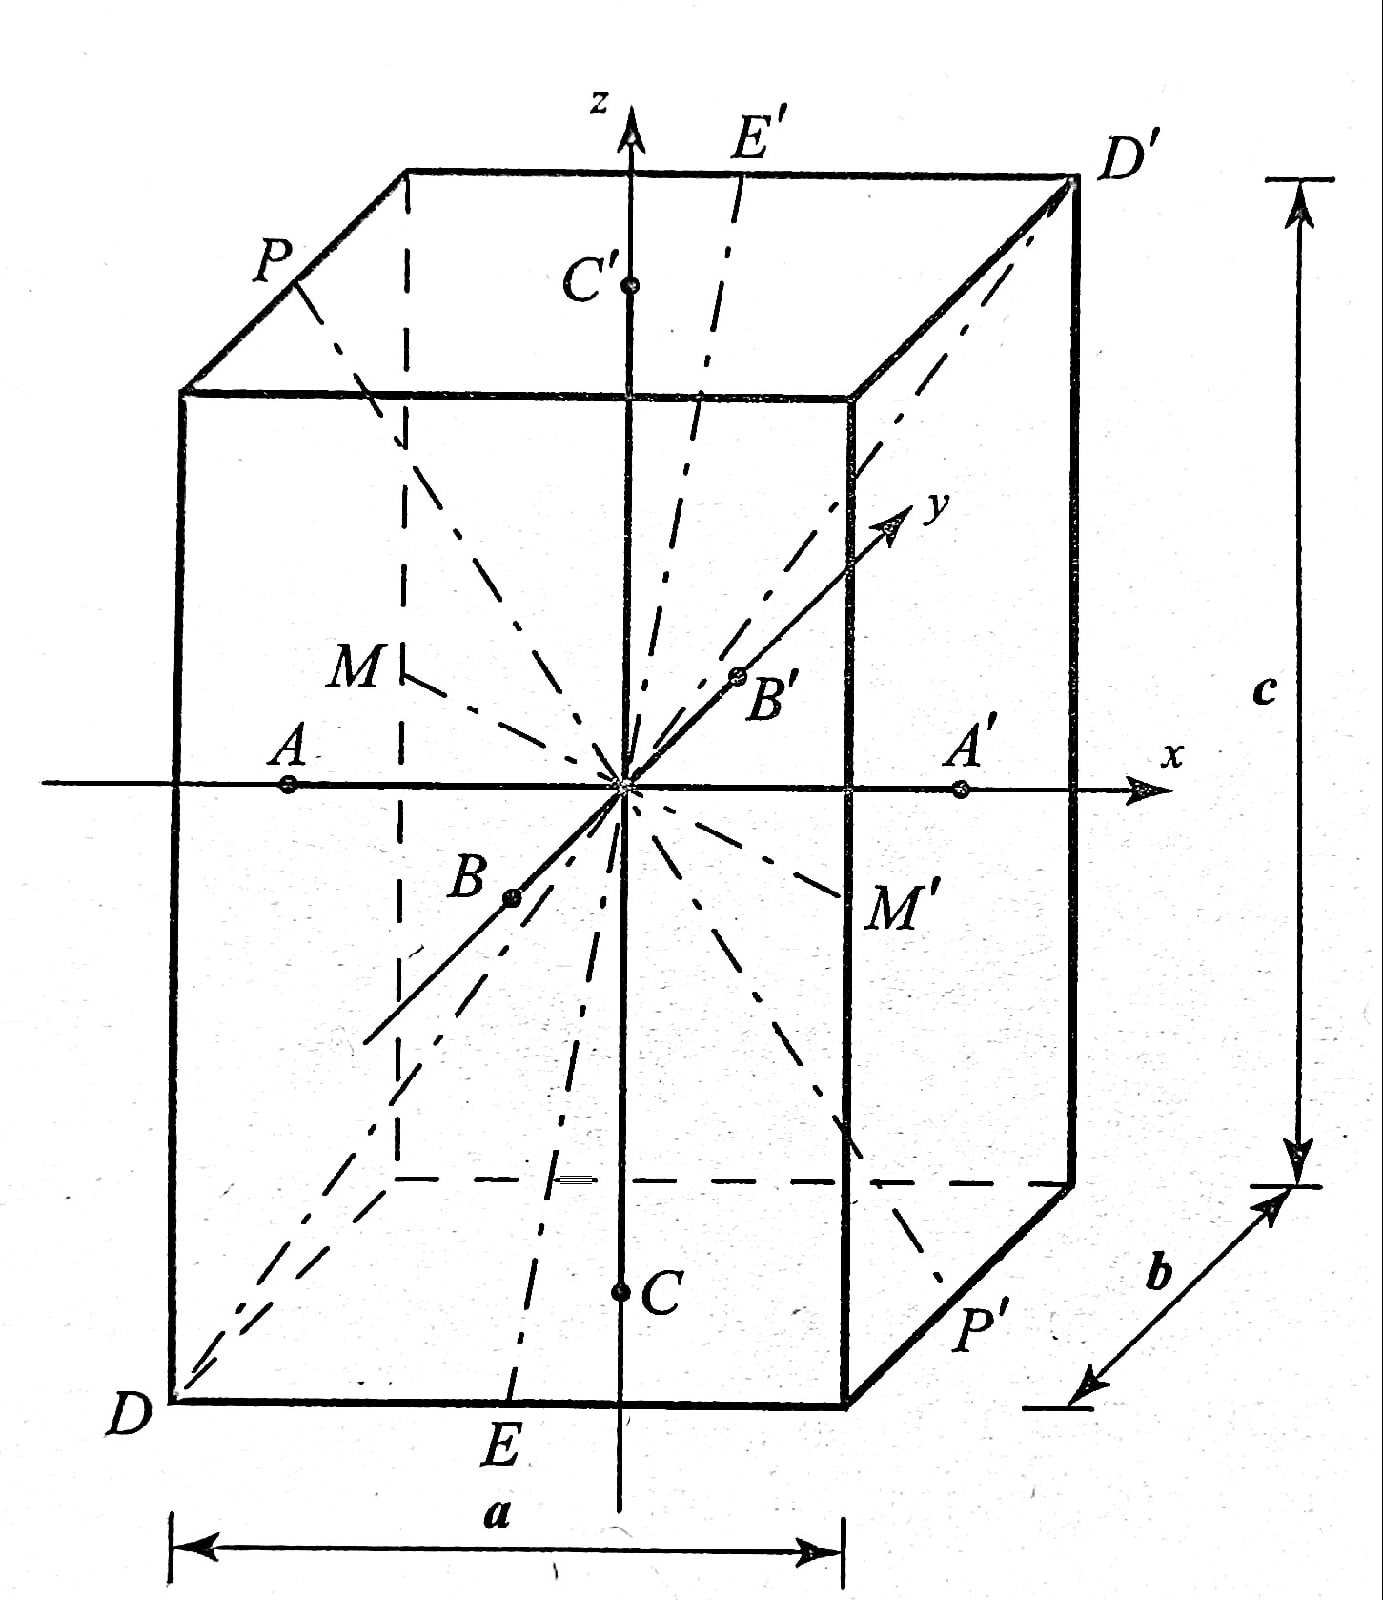
\includegraphics[width=\linewidth]{parallelepiped.jpg}
	\caption{Оси вращения прямоугольного параллелепипеда}
    \label{pic:parallelepiped}
\end{wrapfigure}

Моменты инерции относительно этих осей обозначим $I_x$, $I_y$, $I_z$. Ось $DD'$ составляет с главными осями такие же углы, как и с ребрами $a$, $b$ и $c$. Косинусы этих углов, соотвественно, $\dfrac{a}{d}$, $\dfrac{b}{d}$ и $\dfrac{c}{d}$, где $d$ -- длина диагонали: $d = \sqrt{a^2 + b^2 + c^2}$.

Тогда момент инерции $I_d$ вращения вокруш может быть $DD'$ выражается через главные моменты с помощью следующей формулы:
\begin{equation}
    I_d = I_x\frac{a^2}{d^2} + I_y\frac{b^2}{d^2} + I_z\frac{c^2}{d^2}
\end{equation}

Отсюда получаем соотношение:
\begin{equation}
    (a^2 + b^2 + c^2)I_d = a^2 I_x + b^2I_y + c^2I_z
\end{equation}

Используя связь момента инерции с периодом крутильных колебаний \eqref{eq:period}, получаем соотношеине:

\begin{equation}
    (a^2 + b^2 + c^2)T_d^2 = a^2T_x^2 + b^2T_y^2 + c^2T_z^2
\end{equation}

Из этой формулы следуют также выражения, связывающие моменты инерции относительно осей $EE'$, $MM'$ и $PP'$ с главными моментами инерции. С помощью формулы \eqref{eq:period} и для этих осей получаем выражения для периодов крутильных колебаний:

\begin{eqnarray}
    \label{eq:t_for_e}
    (b^2 + c^2)T_E^2 = b^2T_y^2 + c^2T_z^2 \\
    \label{eq:t_for_p}
    (a^2 + c^2)T_P^2 = a^2T_x^2 + c^2T_z^2\\
    \label{eq:t_for_m}
    (a^2 + b^2)T_M^2 = a^2T_x^2 + b^2T_y^2
\end{eqnarray}

\parag {Ход работы} ~\\

Измерим периоды колебаний куба относительно главных осей, главной диагонали и диагонали, соединяющей противоположные ребра противоположных граней. Результаты занесем в таблицу \ref{tabl:cube}. Для куба была выбрана амплитуда колебаний в $21.5\degree \pm 0.05\degree$.

\begin{table}[!h]
    \centering
    \begin{tabularx}{\textwidth}
        {|C|C|C|C|}
        \hline
        \textbf{\textnumero \quad опыта} & \textbf{Кол-во колебаний $N$} & \textbf{Полное время, сек} & \textbf{Расчитанный период, сек}  \\ \hline
        \multicolumn{4}{|c|}{главная ось} \\ \hline
        \textbf{1 } & 10 & 52.6  & 5.26   \\ \hline
        \textbf{2 } & 10 & 52.42 & 5.242  \\ \hline
        \textbf{3 } & 10 & 52.22 & 5.22   \\ \hline
        \textbf{4 } & 10 & 53.57 & 5.357  \\ \hline
        \textbf{5 } & 10 & 52.32 & 5.232  \\ \hline
        \multicolumn{4}{|c|}{среднее значеине для главной оси: $5.262 \pm 0.099$ сек.} \\ \hline
        \multicolumn{4}{|c|}{главная диагональ} \\ \hline
        \textbf{1 } & 10 & 52.55 & 5.255 \\ \hline
        \textbf{2 } & 10 & 51.89 & 5.189  \\ \hline
        \textbf{3 } & 10 & 52.54 & 5.254 \\ \hline
        \textbf{4 } & 10 & 52.57 & 5.257 \\ \hline
        \textbf{5 } & 10 & 52.26 & 5.226 \\ \hline
        \multicolumn{4}{|c|}{среднее значеине для главной диагонали: $5.236 \pm 0.099$ сек.} \\ \hline
        \multicolumn{4}{|c|}{дополнительная диагональ} \\ \hline
        \textbf{1 } & 10 & 52.21 & 5.221 \\ \hline
        \textbf{2 } & 10 & 53.02 & 5.302 \\ \hline
        \textbf{3 } & 10 & 52.10 & 5.21 \\ \hline
        \textbf{4 } & 10 & 52.73 & 5.273 \\ \hline
        \textbf{5 } & 10 & 52.32 & 5.232 \\ \hline
        \multicolumn{4}{|c|}{среднее значеине для дополнительной диагонали: $5.2476 \pm 0.1$ сек.}\\ \hline
    \end{tabularx}
    \caption{Результаты измерения времени 10 крутильных колебаний для разных осей куба}
    \label{tabl:cube}
\end{table}


\parag{Измерим длину ребра куба}
Длину ребра куба $a$ измерим штангенциркулем. Получим: $a = 9.27 \pm 0.05 ~ см$. Проверим справедливость формул \eqref{eq:t_for_e}, \eqref{eq:t_for_p} и \eqref{eq:t_for_m}.

\parag{Найдем соотвествующие формулы для куба}
Для начала заметим, что косинусы углов между главной диагональю куба и каждой из основных осей равны в силу симметрии друг другу и равны $cos(\alpha) = \dfrac{1}{\sqrt{3}}$.

Тогда для периода крутильных колебаний относительно главной диагонали куба получим формулу 
\begin{equation}
     T_d = \sqrt{\frac{a^2T_x^2 + a^2T_y^2 + a^2T_z^2}{3a^2}}
\end{equation}

Подставляя значения из таблицы в формулу выше получим, что $T_{d_{расчит.}} \approx 5.262 \pm 0.087$. Полученное экспериментрально значение  $T_{d_{эспер.}} \approx 5.236 \pm 0.099$, что хорошо соотносится с экспериментом.

Аналогичным образом получим формулу для дополнительной оси:
\begin{equation}
    T_{dd} = \sqrt{\frac{a^2T_y^2 + a^2T_z^2 }{2a^2}}
\end{equation}

Подставляя значения из таблицы в формулу выше получим, что $T_{{dd}_{расчит.}} \approx 5.248 \pm 0.09$. Полученное экспериментрально значение  $T_{{dd}_{эспер.}} \approx 5.2476 \pm 0.09$, что еще лучше соотносится с экспериментом.

\parag{Перейдем к параллелепипеду}
Измерим параметры параллелепипеда и рассчитаем длину его диагонали. Результат занесем в таблицу \ref{tabl:parallelepiped_size}.

\begin{table}[!h]
    \centering
    \begin{tabularx}{\textwidth}
        {|C|C|}
        \hline
        a & $10.03 \pm 0.05$ см. \\ \hline
        b & $5.03 \pm 0.05$ см. \\ \hline
        c & $15.03 \pm 0.05$ см. \\ \hline
        d & $18.75 \pm 0.005$ см. \\ \hline
    \end{tabularx}
    \caption{Результаты измерения параметров параллелепипеда}
    \label{tabl:parallelepiped_size}
\end{table}

\parag{Проведем серию экспериментов по расчету времени крутильных колебаний относительно нескольких осей параллелепипеда} 
Для параллелепипеда была выбрана амплитуда колебаний в $31.5\degree \pm 0.05\degree$. Результат занесем в таблицу \ref{tabl:parallelepiped_experiments}.

\begin{table}[h]
    \centering
    \begin{tabularx}{\textwidth}
        {|C|C|C|C|}
        \hline
        \textbf{\textnumero \quad опыта} & \textbf{Кол-во колебаний $N$} & \textbf{Полное время, сек} & \textbf{Расчитанный период, сек}  \\ \hline
        \multicolumn{4}{|c|}{ось $AA'$} \\ \hline
        \textbf{1 } & 10 & 62.35 & 6.235    \\ \hline
        \textbf{2 } & 10 & 62.82 & 6.282   \\ \hline
        \textbf{3 } & 10 & 62.33 & 6.233    \\ \hline
        \textbf{4 } & 10 & 62.68 & 6.268   \\ \hline
        \multicolumn{4}{|c|}{среднее значение для оси: $6.2545 \pm 0.099$ сек.} \\ \hline
        \multicolumn{4}{|c|}{ось $BB'$} \\ \hline
        \textbf{1 } & 10 & 64.11 &  6.411 \\ \hline
        \textbf{2 } & 10 & 64.04 &  6.404  \\ \hline
        \textbf{3 } & 10 & 64.14 &  6.414 \\ \hline
        \textbf{4 } & 10 & 64.27 &  6.427 \\ \hline
        \multicolumn{4}{|c|}{среднее значение для оси $6.414 \pm 0.099$ сек.} \\ \hline
        \multicolumn{4}{|c|}{ось $CC'$} \\ \hline
        \textbf{1 } & 10 & 56.05 & 5.605 \\ \hline
        \textbf{2 } & 10 & 55.77 & 5.577 \\ \hline
        \textbf{3 } & 10 & 55.72 & 5.572 \\ \hline
        \textbf{4 } & 10 & 55.23 & 5.523 \\ \hline
        \multicolumn{4}{|c|}{среднее значение для оси $5.569 \pm 0.099$ сек.} \\ \hline
        \multicolumn{4}{|c|}{ось $DD'$} \\ \hline
        \textbf{1 } & 10 & 59.85 & 5.985 \\ \hline
        \textbf{2 } & 10 & 59.64 & 5.964 \\ \hline
        \textbf{3 } & 10 & 60.12 & 6.012 \\ \hline
        \textbf{4 } & 10 & 59.32 & 5.932 \\ \hline
        \multicolumn{4}{|c|}{среднее значение для оси $5.973 \pm 0.099$ сек.} \\ \hline
        \multicolumn{4}{|c|}{ось $EE'$} \\ \hline
        \textbf{1 } & 10 & 57.43 & 5.743 \\ \hline
        \textbf{2 } & 10 & 57.45 & 5.745 \\ \hline
        \textbf{3 } & 10 & 58.29 & 5.829 \\ \hline
        \textbf{4 } & 10 & 57.58 & 5.758 \\ \hline
        \multicolumn{4}{|c|}{среднее значение для оси $5.769 \pm 0.099$ сек.} \\ \hline
        \multicolumn{4}{|c|}{ось $PP'$} \\ \hline
        \textbf{1 } & 10 & 58.20 & 5.820 \\ \hline
        \textbf{2 } & 10 & 58.23 & 5.823 \\ \hline
        \textbf{3 } & 10 & 58.05 & 5.805 \\ \hline
        \textbf{4 } & 10 & 58.25 & 5.825 \\ \hline
        \multicolumn{4}{|c|}{среднее значение для оси $5.818 \pm 0.099$ сек.} \\ \hline
        \multicolumn{4}{|c|}{ось $MM'$} \\ \hline
        \textbf{1 } & 10 & 59.32 & 5.932 \\ \hline
        \textbf{2 } & 10 & 59.47 & 5.947 \\ \hline
        \textbf{3 } & 10 & 59.29 & 5.929 \\ \hline
        \textbf{4 } & 10 & 59.01 & 5.901 \\ \hline
        \multicolumn{4}{|c|}{среднее значение для оси $5.927 \pm 0.099$ сек.} \\ \hline
    \end{tabularx}
    \caption{Результаты измерения времени 10 крутильных колебаний для разных осей параллелепипеда}
    \label{tabl:parallelepiped_experiments}
\end{table}


\parag{Проверим верность формул}
 Используя значения из таблицы, а также измеренные размеры параллелепипеда, проверим справедливость формул \eqref{eq:t_for_e}, \eqref{eq:t_for_p} и \eqref{eq:t_for_m}.

Расчитаем период крутильных колебаний для каждой из осей: $MM'$, $EE'$, $PP'$ и $DD'$:
\begin{eqnarray}
    T_{E} = \sqrt{\frac{(b^2T_y^2 + c^2T^2_z)}{(b^2 + c^2)}}\\
    T_{P} = \sqrt{\frac{(a^2T_x^2 + c^2T^2_z)}{(a^2 + c^2)}}\\
    T_{M} = \sqrt{\frac{(a^2T_x^2 + b^2T^2_y)}{(a^2 + b^2)}}\\
    T_{D} = \sqrt{\frac{(a^2T_x^2 + b^2T^2_y + c^2T^2_z)}{(a^2 + b^2 + c^2)}}
\end{eqnarray}

Подставим значения из таблицы и получим:
\[
    T_{E} = 5.659~ с. \pm 0.23\\
\]
\[
    T_{P} = 5.788~ c. \pm 0.11\\
\]
\[
    T_{M} = 6.286~ c. \pm 0.117\\
\]
\[
    T_{D} = 5.836~ c. \pm 0.57\\
\]

Как видно, расчитанные значения с высокой точностью сходятся со значениями из таблицы. Это подтверждает верность формул, приведенных выше.

\parag{Построим проекции эллипсоида инерции для параллелепипеда}
Чтобы построить проекции эллипсоида на главные плоскости, воспользуемся фактом, что величина $r = \dfrac{1}{\sqrt{T^2 - T^2_р}}$ пропорциональна расстоянию от центра масс тела до точки пересечения эллипсоида с данной осью. Рассчитаем данную величину для каждой из главных осей:
\[
    r_{x} = 0.209 \pm 0.001\\
\]
\[
    r_{y} = 0.200 \pm 0.001\\
\]
\[
    r_{z} = 0.261 \pm 0.001\\
\]

Поскольку данные коэффициенты только пропорциональны полуосям эллипса, для наглядности чертежа домножим каждый из них на 15.

Построим эллипсоид инерции в разных сечениях.
\begin{figure}
    \begin{subfigure}{\linewidth}
    \centering
    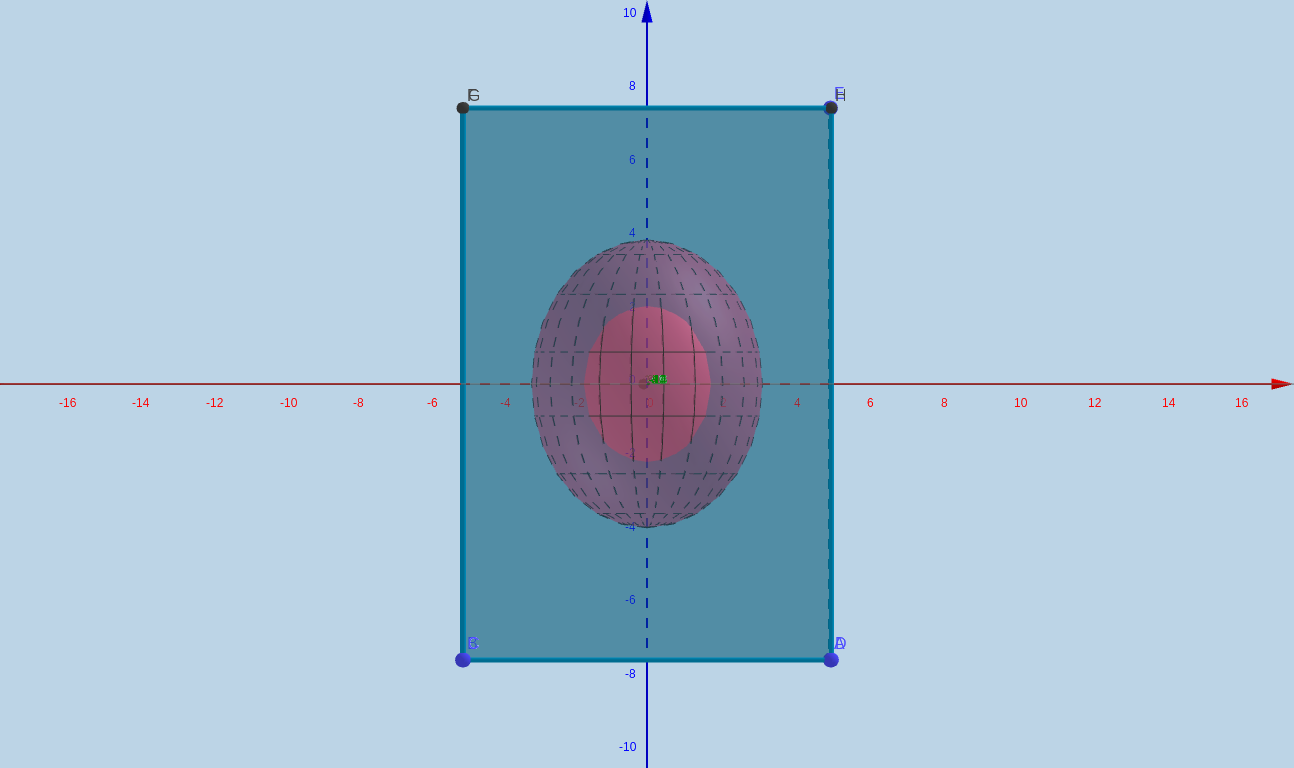
\includegraphics[width=.75\linewidth]{ellipsis1.png}
	\caption{Эллипсоид инерции в сечении yz}
    \end{subfigure}\par\medskip
    \begin{subfigure}{\linewidth}
    \centering
    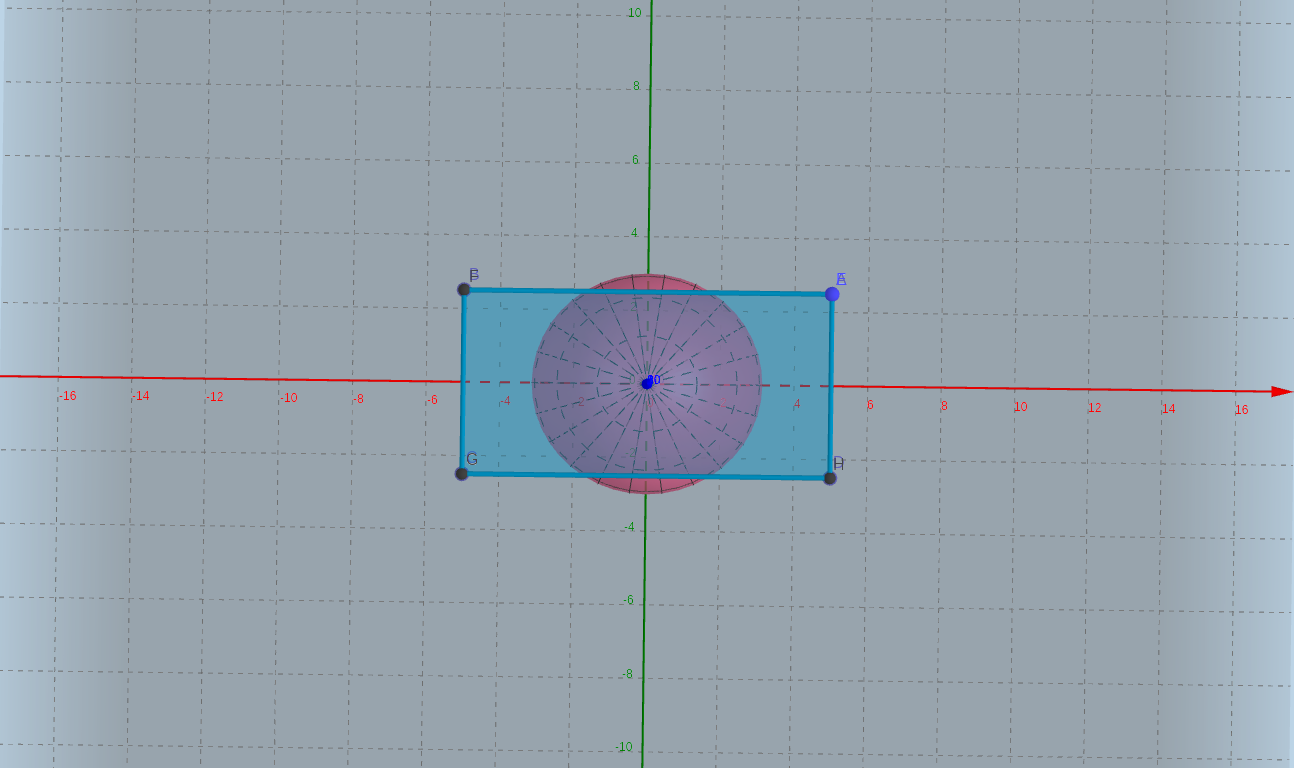
\includegraphics[width=.75\linewidth]{ellipsis2.png}
	\caption{Эллипсоид инерции в сечении xy}
    \end{subfigure}\par\medskip
    \begin{subfigure}{\linewidth}
    \centering
    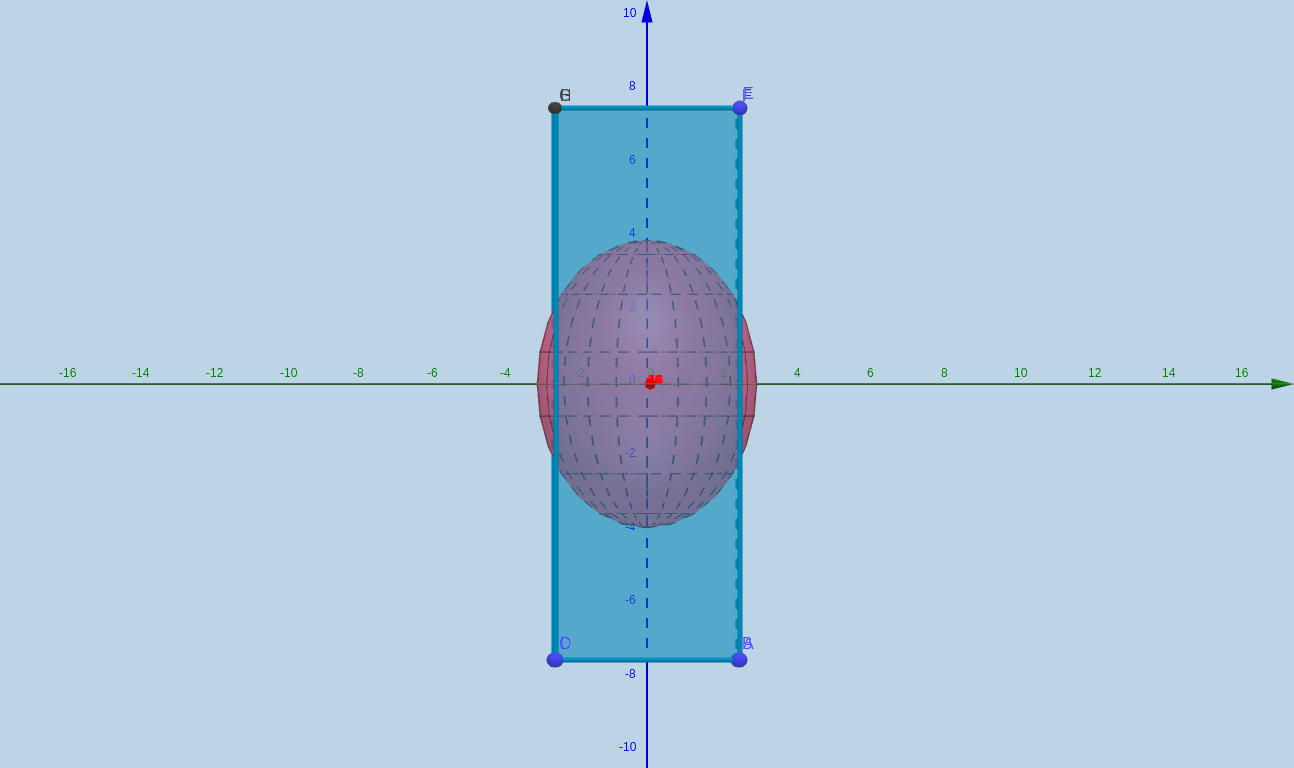
\includegraphics[width=.75\linewidth]{ellipsis3.png}
	\caption{Эллипсоид инерции в сечении xz}
    \label{pic:graph}
    \end{subfigure}\par\medskip
	\caption{Эллипсоид инерции в различных сечениях}
\end{figure}

\begin{figure}
    \centering
    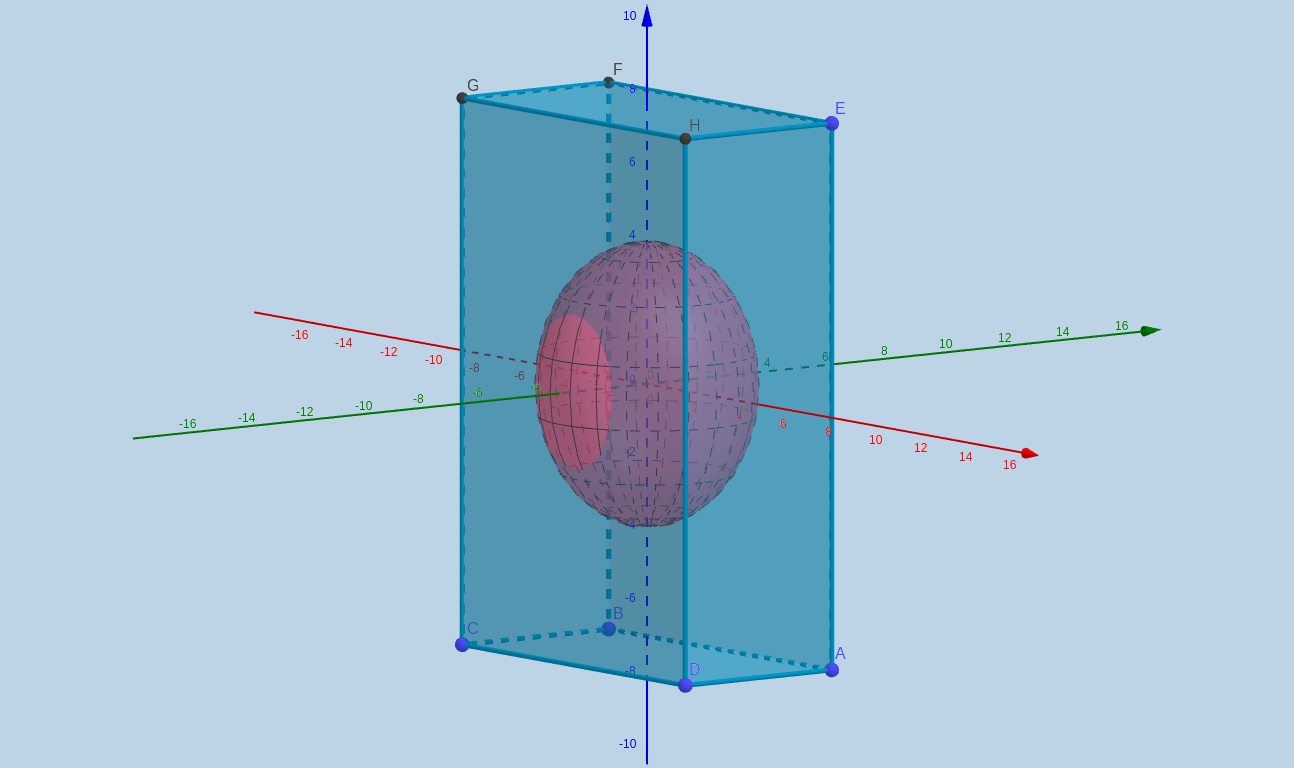
\includegraphics[width=15cm]{ellipsis4.png}
	\caption{Эллипсоид инерции в трехмерном формате}
    \label{pic:graph}
\end{figure}

\parag {Заключение} ~\\
В процессе лабораторной работы была экспериментально доказана верность формул, позволяющих расчитывать момент инерции (а следовательно и период крутильных колебаний) относительно произвольной оси, проходящей через центр масс тела, используя только моменты инерций основных осей тела. Кроме того, был построен эллипсоид инерции для тела, моменты которого измерялись.
\end{document} 
